\AddToShipoutPictureBG*{
    \AtPageLowerLeft{
        
\includegraphics[width=\paperwidth,height=\paperheight]{chapters/chapter2.jpg}
    }
}


\decorate{缘起}

\pagestyle{empty}


\begin{center}
    \vspace*{1.5cm}
    \color{white}
    {
    \Large
    一场未经编排的雪 \par \vspace*{0.4cm}
    让两粒漂泊的逗号 \par   \vspace*{0.4cm}
    在茫茫人海中 \par\vspace*{0.4cm}
    突然站成一对引号 \par\vspace*{0.4cm}
    在十二月的寂静里\par\vspace*{0.4cm}
    划出温暖的弧度 \par\vspace*{0.4cm}
    我们呼出的白雾 \par\vspace*{0.4cm}
    正在完成云朵的叙事 \par \vspace*{0.4cm}
    此刻世界如此轻盈 \par \vspace*{0.4cm}
    像刚刚诞生的童话 \par \vspace*{0.4cm}
    连误入站台的蝴蝶 \par \vspace*{0.4cm}
    都带着宿命的征兆
    }
    \vfill
    \makefoot
\end{center}

\card{covers/cover1.jpg}{A}{永远在你身边}{Always by your side}

\setstyle{Always by your side}

\subtitle{北京初雪——故事的开始}

\large
\begin{spacing}{2}
    北京的初雪，在我一遍遍的预告里，终于落了下来。

    窗外一泛起那种特殊的、灰白而明亮的光，我的心就跳快了。那是只有雪天才有的光线，柔和而清冷，把整个世界都镀上一层静谧的银白。
    我推开窗，寒风裹挟着细碎的雪花扑面而来，落在睫毛上，瞬间融化成微凉的水珠。

    \begin{figure}[!htbp]
        \centering
        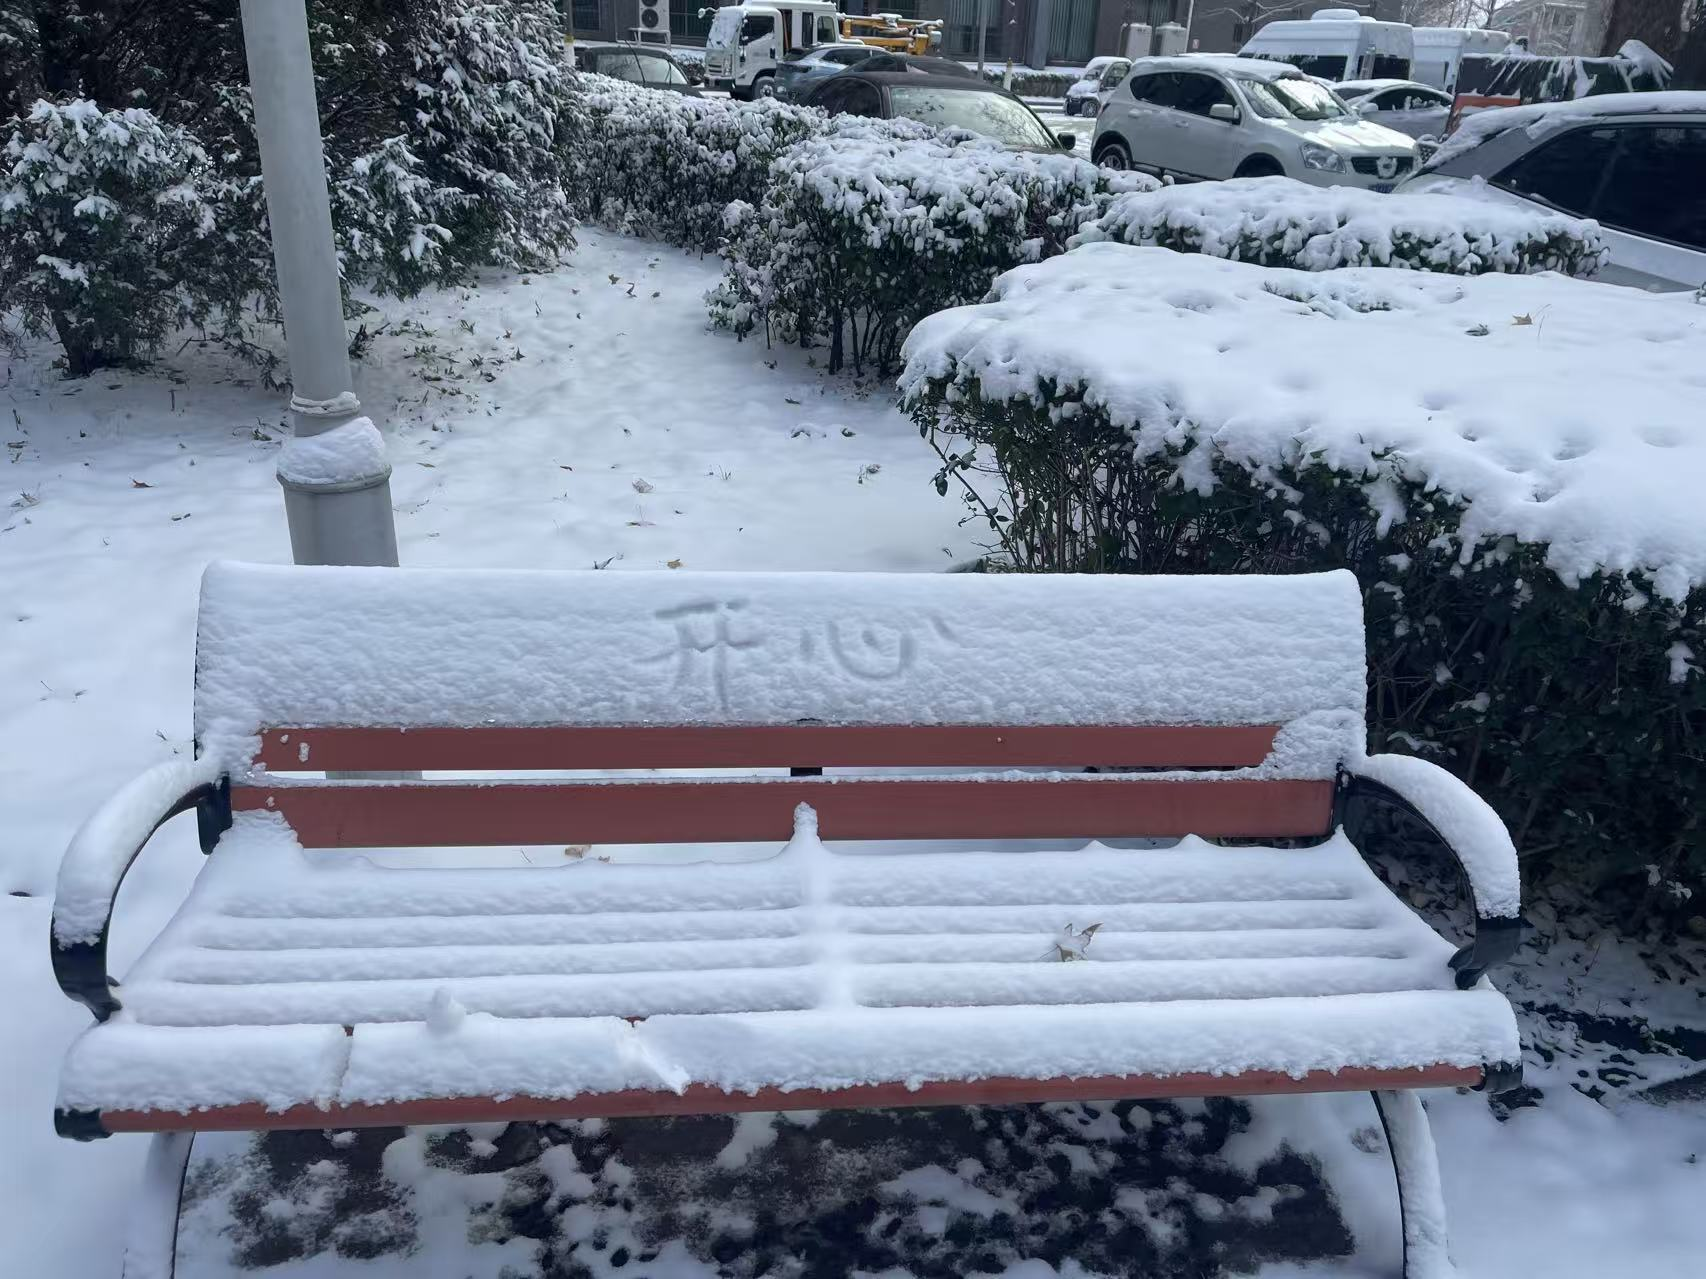
\includegraphics[width=\textwidth]{figures/articles/01-1.jpg}
        \caption*{\small{北京二零二三年的初雪}}
    \end{figure}
    
    镜头缓缓扫过覆白的车顶、灌木丛，以及地上那层薄薄的、却足以让整个世界安静下来的雪。
    每一片雪花都像是天空写给人间的情书，轻轻覆盖了城市的喧嚣。远处的树枝被积雪压弯了腰，
    偶尔有麻雀飞过，抖落一树晶莹。

    还记得我那天早上去上课滑倒了嘛。那一刻的惊慌失措，让我像个笨拙的孩子。
    路面上的薄冰像是生活开的小玩笑，而我恰好是那个笑点。我还以为你也要笑话我哈哈哈，
    毕竟连我自己都觉得又好气又好笑。

    可你没有。你第一时间发来消息：“疼不疼？有没有受伤？别着凉了。”
    简短的几句话，却让我在寒冷的雪天里感受到了最深的暖意。原来被一个人真心惦记着，
    是这样的感觉——即使相隔千里，关怀却能穿越山河，精准地落在心尖上。

    不过这个冬天你运气也似乎不太好，屡次感冒，被迫喝那苦涩的中药。
    我现在似乎可以想象着你在那端，捧着温热的药碗，像个不肯吃药的孩子。

    但没关系，有我在。虽然我们之间隔着一两千公里的距离，但爱意从来不会被地理的刻度所限制。
    我在这里，在每一个你需要的时候，用文字、用声音、用所有能抵达你的方式，陪伴着你。
    就像这初雪，虽然落在不同的城市，但我们仰望的是同一片天空，感受的是同一种寒冷，怀揣的是同一份温暖。

    雪花还在静静飘落，覆盖了行人留下的脚印，也覆盖了时光里的所有遗憾。我想，
    每一片雪花都是天空写给大地的诗，而我们的故事，就是这首诗里最动人的韵脚。

    \bottomtext{“雪花是信使，传递相遇的讯号”}
\end{spacing}

\card{covers/cover2.jpg}{B}{和你在一起}{Be with you}

\setstyle{Be with you}

\subtitle{吉安火车站——月台与黄昏的约定}

\large
\begin{spacing}{2}
    吉安站的广场上，浸在2024年2月黄昏时一种半明半暗的蓝调里。
    空气凛冽，呵出的白气迅疾地消散，像我狂跳不止的心。

    我站在广场的天桥上四处张望，每一辆公交车都像是载着你的工具，每一个脚步声都像敲在心跳的鼓点上。
    你突然出现在我身后，我也一眼就认出了你——和视频里一样，又完全不一样，
    那天你穿的很美，哑光面的黑色棉袄，那条黑色牛仔裤紧贴着你的腿部线条，
    从宽厚的棉袄下延伸而出，利落得惊人，踩着那双黑色板鞋快步走过，你并不刻意追求精致，
    但这一身黑却因你从容的神情，显得洒脱又高级。

    \begin{figure}[!htbp]
        \centering
        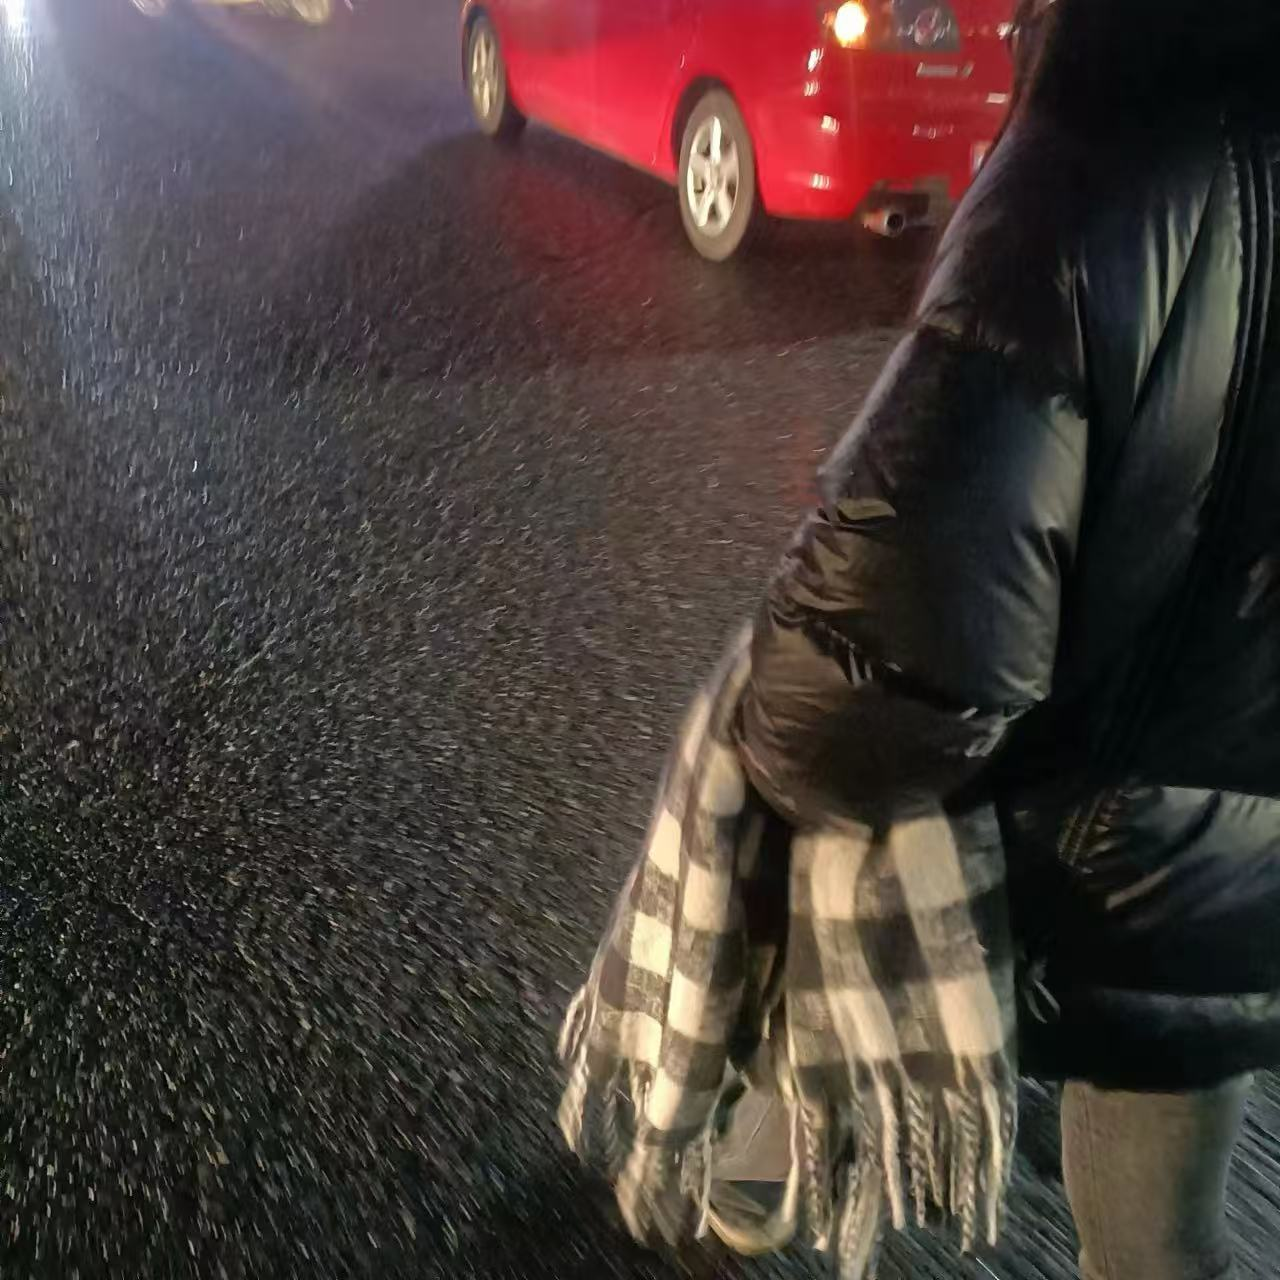
\includegraphics[width=0.4\textwidth]{figures/articles/01-2.jpg}
        \caption*{\small{你的全身装扮}}
    \end{figure}

    你站在清冷的微光里，像整个世界唯一的热源。没有预演，没有犹豫，在人流稀疏的广场上，
    你率先打破尴尬，我们自然而然地拥抱在一起。那个拥抱，用力得像要把之前所有屏幕里的思念，
    都挤压进彼此的骨血里。你身上带着室外清新的寒气，而拥抱的核心，是滚烫的。

    分开一点，只是为了看清你的脸。你的眼睛亮得惊人，里面有我的倒影，也有初升旭日碎金般的光。
    然后，我们坐在广场上的长椅时，你吻了我。那不是电影里缠绵悱恻的长吻。
    它是一个轻柔的、带着冬日凉意的触碰，却像一道温暖的闪电，击穿了所有因陌生而产生的藩篱。
    世界只剩下唇上那片柔软的雪花，正在慢慢融化。

    \begin{figure}[!htbp]
        \centering
        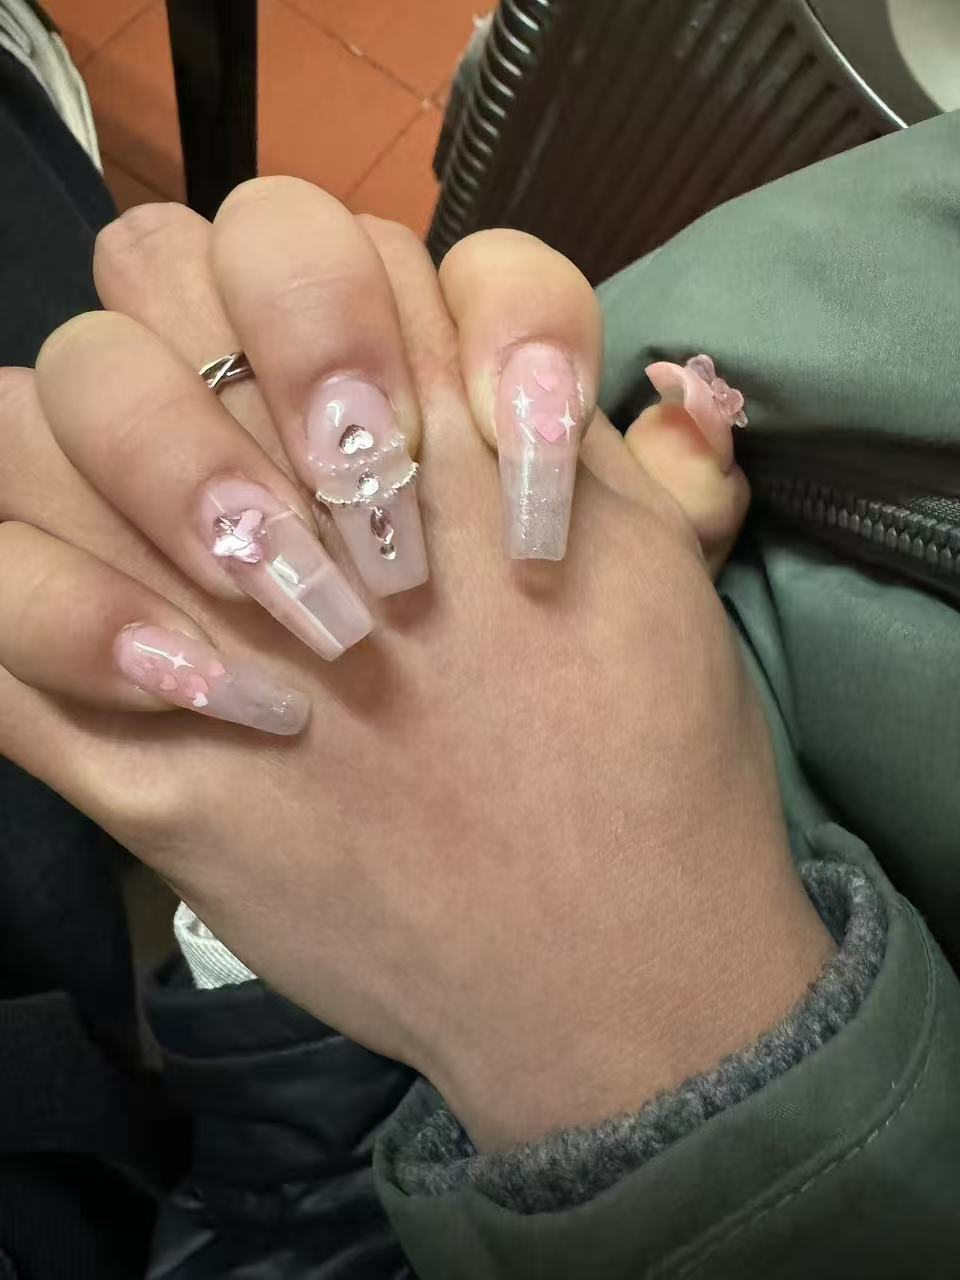
\includegraphics[width=0.4\textwidth]{figures/articles/01-3.jpg}
        \caption*{\small{我们十指相扣就像握住了全世界}}
    \end{figure}

    “冷不冷？”我低声问，我的手很自然地找到你的手，紧紧握住。你摇摇头，又点点头，自己都忍不住笑了。
    是冷的，手是冰的，脸是冻的。可心里却烧着一团火，从心脏一直暖到指尖。
    走出站口，空气中飘来一股熟悉的、属于人间烟火的焦香。旁边有个小摊，铁板上滋滋啦啦地烤着香肠。
    “给你买根烤肠吧。”我说。那根烤肠，在寒冷的冬天冒着粗犷而诱人的热气。
    你仔细地吹了吹，才咬下一口，我们就站在吉安站的广场上，分享着那根二块钱的烤肠。
    我看着你被烫得微微蹙眉的样子，笑得像个孩子。

    那一刻，我们的爱情，从云端的诗篇，稳稳地落在了地上。
    它有了体温——是拥抱的力度，是亲吻的清凉，是紧紧相扣的十指，
    是2024年2月25日，吉安火车站，一个星光即将完全消散的黄昏。

    月台见证了我们的奔赴，我们十指紧扣，成了我们第一次见面，最滚烫、最扎实的注脚。
    
    \bottomtext{“黄昏·月台·约定”}
\end{spacing}

\card{covers/cover3.jpg}{C}{永远珍惜你}{Cherish you forever}

\setstyle{Cherish you forever}


\subtitle{鼓楼——时光走漏了风声}

\large
\begin{spacing}{2}
    北京的下午，阳光斜斜地照下来，把行人的影子拉得好长。
    我们混在游客里，沿着鼓楼红墙的根儿走着，墙砖斑斑驳驳，缝隙里都是岁月。

    人实在太多了，喧闹声像一锅煮沸的水。胡同里，光阴仿佛都走得慢了些。
    我们并肩靠在那面历经风雨的红墙上，谁也没有说话。
    砖石传来一种沉稳的、恒久的凉意，透过厚厚的衣料，熨帖在背上。

    \begin{figure}[!htbp]
        \centering
        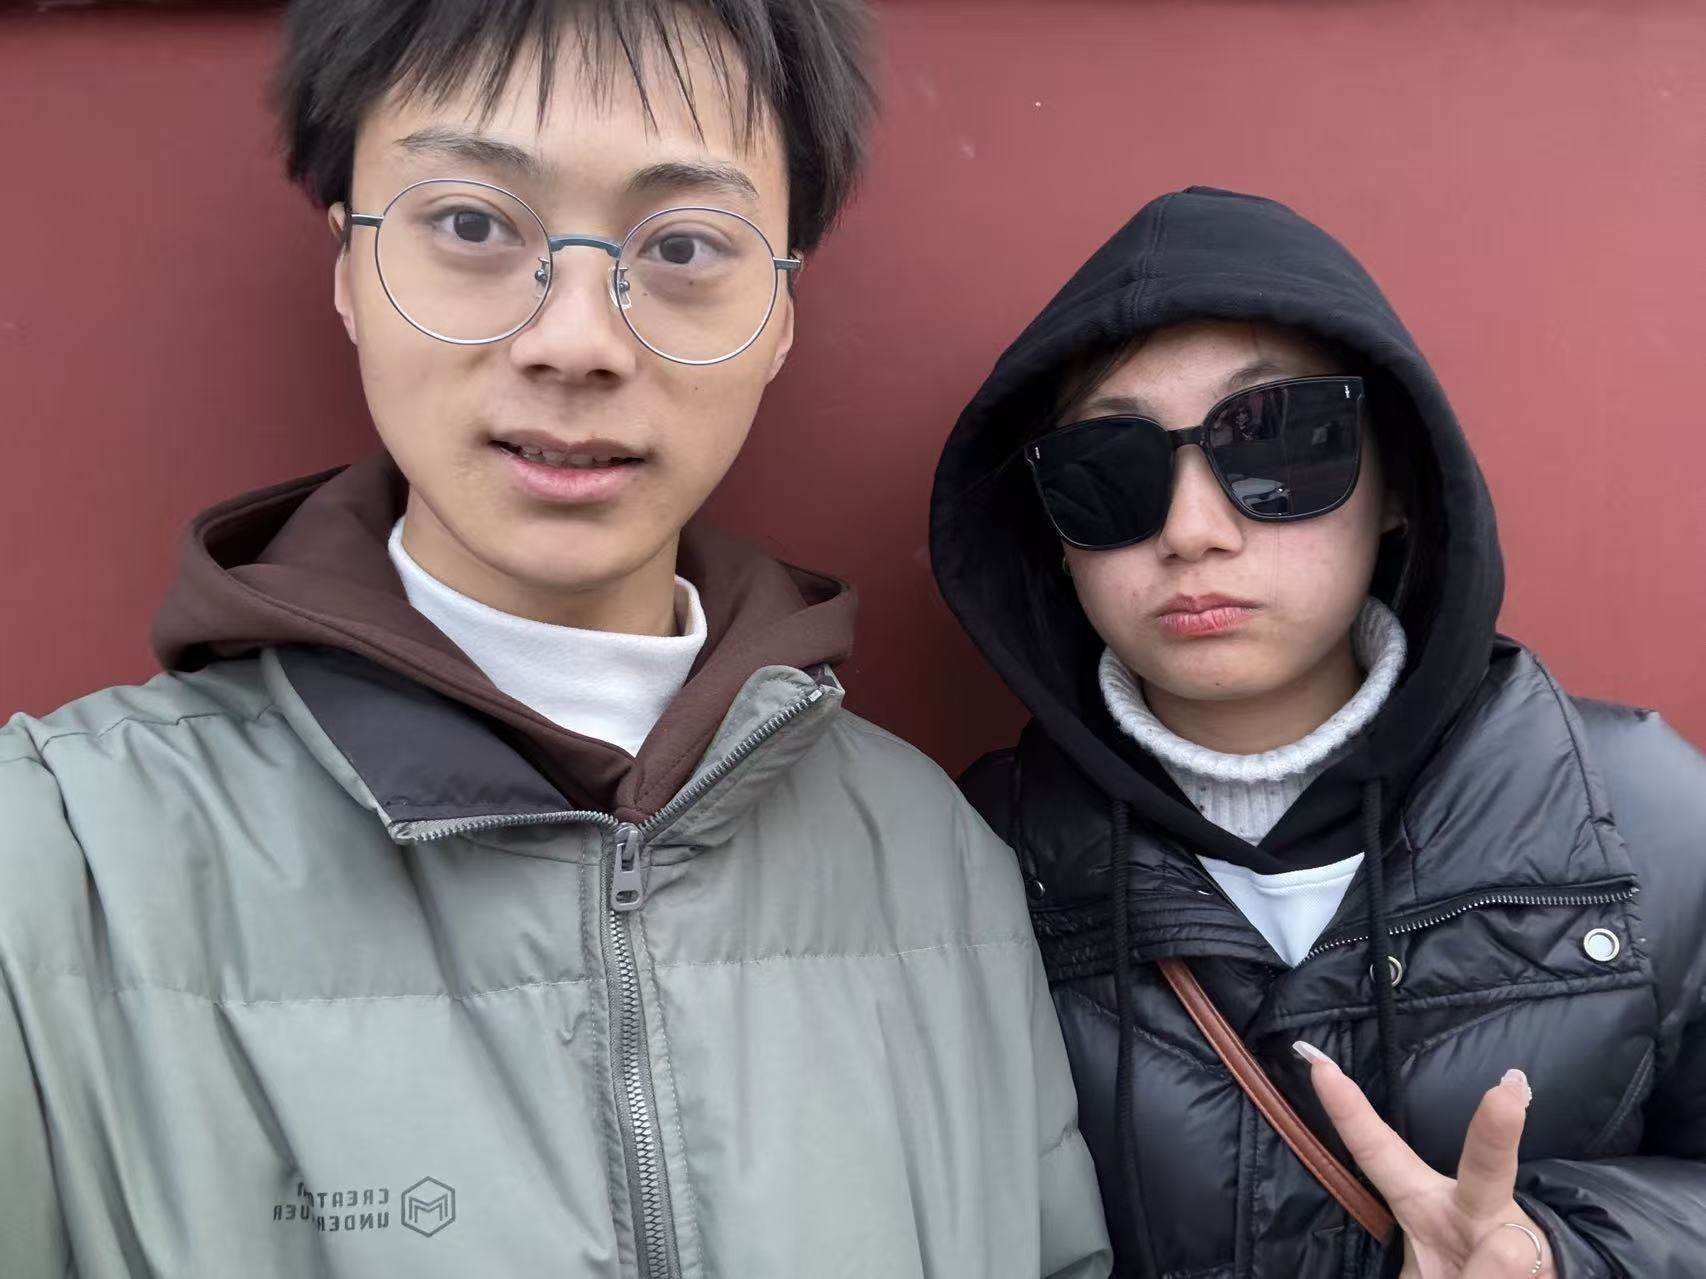
\includegraphics[width=\textwidth]{figures/articles/01-4.jpg}
        \caption*{\small{2024年2月28日午后于鼓楼}}
    \end{figure}

    我们就这样走在人山人海的鼓楼街道，那一天没有夕阳，但我与你心跳共振着。
    那一刻，我忽然觉得，鼓楼这座几百岁的老人，或许并非我们想象的那样沉默。
    它只是说得慢，说得沉。它把故事都藏在风里，藏在砖缝的青苔里，藏在这一声声暮鼓里。
    而此刻，它或许看见了两个靠在一起的年轻身影，看见了他们之间无声流淌的温情。
    它觉得这情景很好，值得被记住。

    你什么也没说，只是把我的手握得更紧一些，我感受着来自掌心的温暖，
    我们没有被写进史书的宏愿，只有此刻背靠着一整部历史的浪漫。

    \bottomtext{“你是我心跳的节拍，呼吸的旋律”}

\end{spacing}

\card{covers/cover4.jpg}{D}{温柔地和你说晚安}{Dear,good night}

\setstyle{Dear,good night}

\subtitle{什刹海——冰面与云的倒影}

\large
\begin{spacing}{2}
    那日的什刹海，没有传说中烧透半边天的绚丽晚霞。
    天色是一种均匀的、沉静的灰蓝，像一块磨砂的玻璃，温和地覆盖在冻结的湖面上。

    \begin{figure}[!htbp]
        \centering
        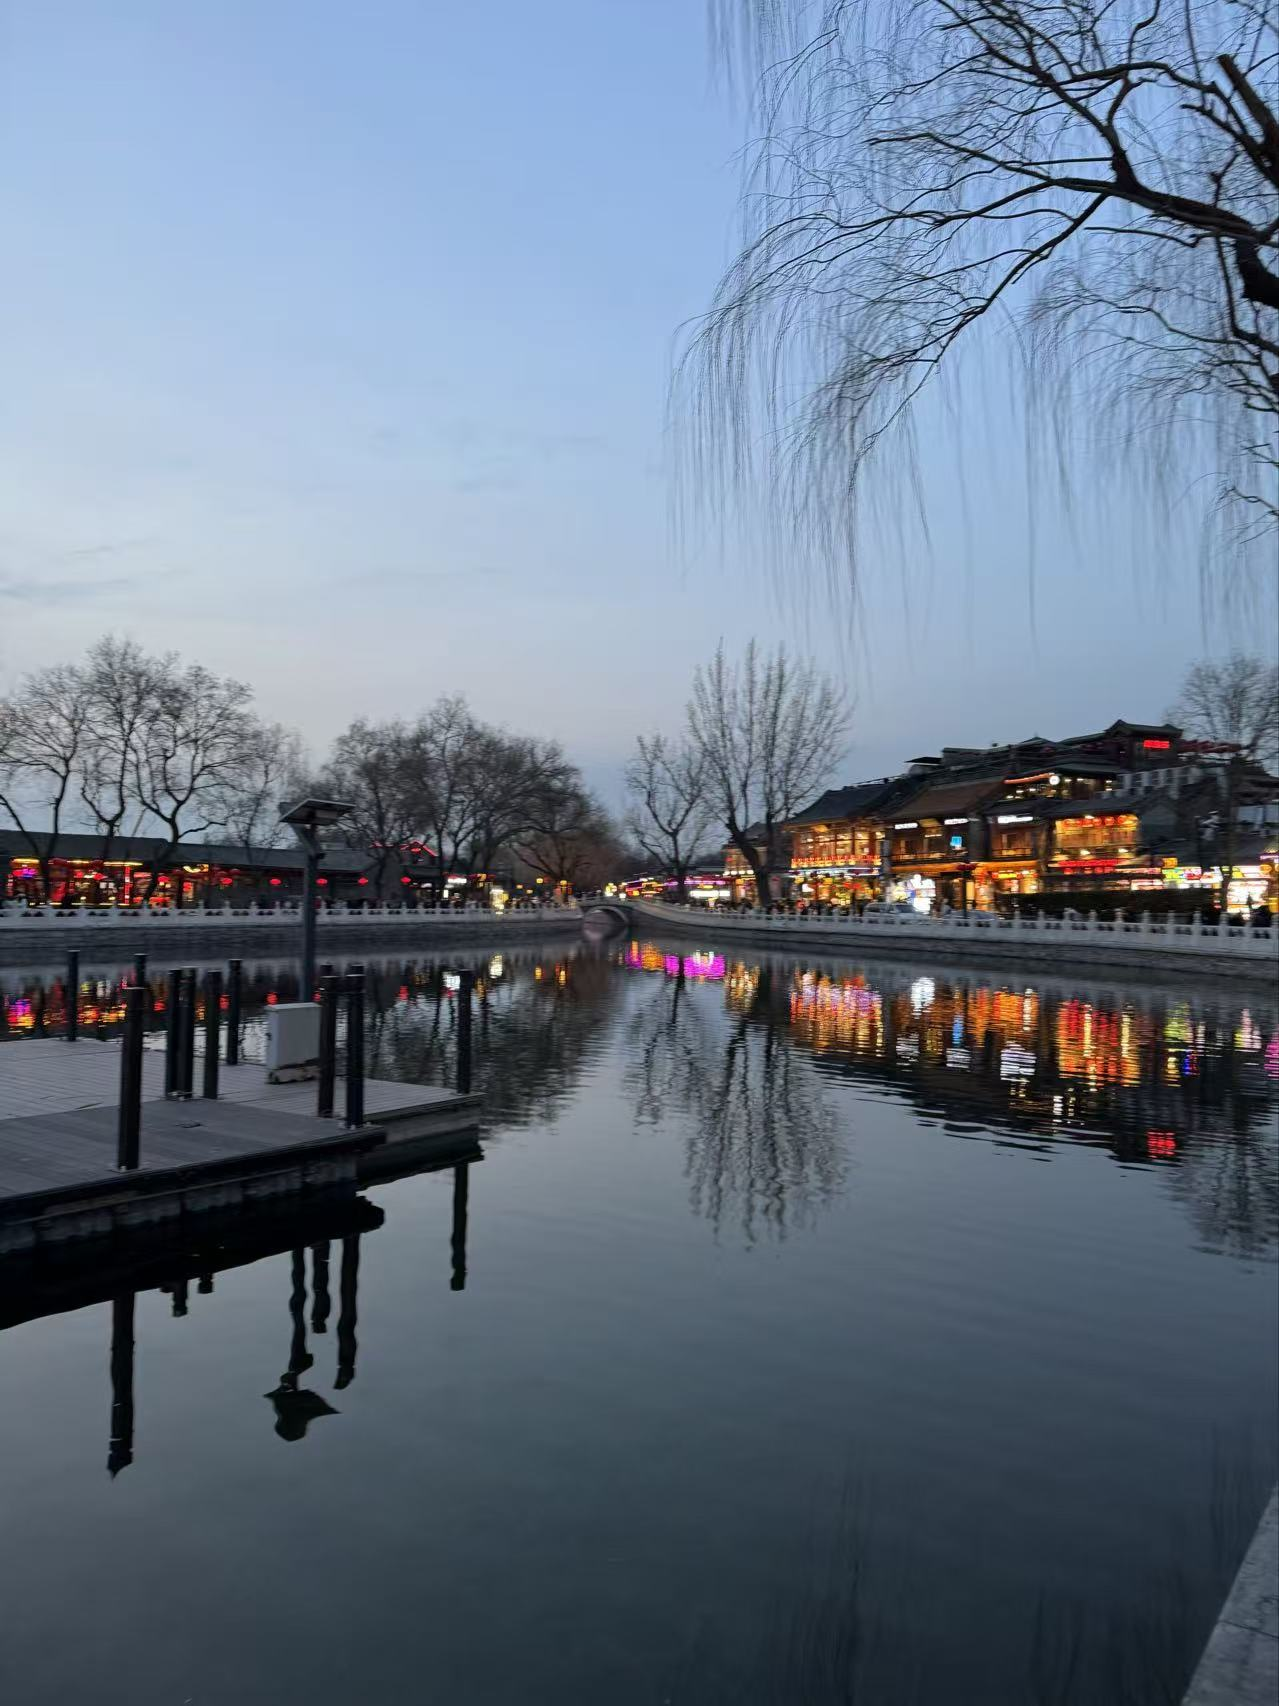
\includegraphics[width=0.4\textwidth]{figures/articles/01-6.jpg}
        \caption*{\small{什刹海冬日景象}}
    \end{figure}

    我们沿着湖岸慢慢地走。冬日萧索，树枝是清瘦的笔触，在水墨画般的天空里勾勒出疏朗的线条。
    岸边的垂柳，褪去了春夏的浓丽，只剩下柔韧的枝条，在微冷的空气里偶尔轻颤。

    人不多，世界显得很安静。我们的交谈也是安静的，像怕惊扰了这片天地固有的节奏。说的无非是些琐碎的日常，偶尔也沉默。
    沉默的时候，就只听得到彼此的脚步声，和从湖面深处隐约传来的、冰层凝结或消融的细微声响。

    我低头看那冰面。它并非透明的，而是一种浑厚的、乳白色的质地，
    像一块巨大的、未经打磨的汉白玉。奇妙的是，它将整个天空都收纳了进来，
    那均匀的灰蓝色调，以及偶尔飘过的、絮状的浅云，都分毫不差地映在上面。
    我们走在岸上，却也像走在云端。我握紧你的手，不需要再多言语了。
    这种虚幻又切实的浪漫，比任何确定的夕阳都更让我们着迷。它留给我们的想象是无尽的。
    天光渐渐暗下去，那均匀的灰蓝色调慢慢沉淀，转为更深的黛蓝。岸边的红灯笼一盏接一盏地亮起来，
    它们暖黄的光晕，并不试图照亮整个湖面，只温柔地染亮了自己脚下的一小方土地与水岸。

    走得有些累了，我们便在湖边一张旧长椅上坐下。眼前是朦胧的灯火与吵闹的酒吧声，身后是无限开阔的、冰与云交融的秘境。
    那一刻，世界仿佛只剩下我们，和这一整片安静的、倒映着天空的冰面。
    我转过头看你，眼睛里有灯笼映出的、小小的光点。它们比天上任何一颗星星都亮。

    \begin{figure}[!htbp]
        \centering
        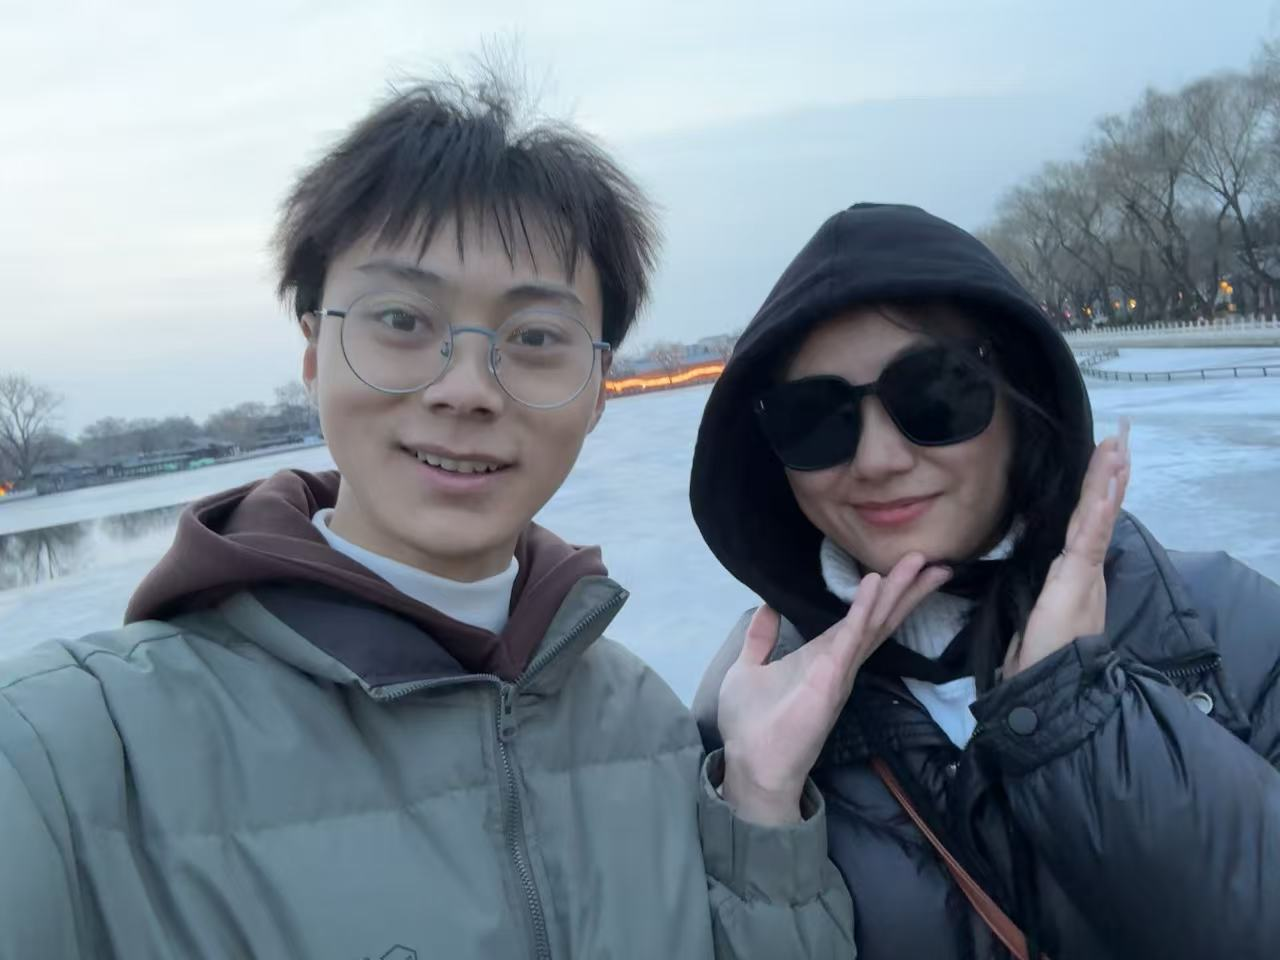
\includegraphics[width=0.6\textwidth]{figures/articles/01-5.jpg}
        \caption*{\small{2024年2月28日傍晚于什刹海}}
    \end{figure}

    一个吻，在那张面向冰湖的长椅上，自然而然地发生了。
    它很轻，带着冬夜的凉意，却又无比温热，像灯火融化了小小的一隅寒冰。
    它不像吉安火车站那个吻那般带着激动的战栗，而是在漫长的漫步与沉默的陪伴后，
    一次水到渠成的靠岸。我们在那片无垠的灰蓝背景下亲吻，仿佛我们的剪影，
    也一同映入了那面巨大的、天空的镜子里。

    \bottomtext{“浮世三千，吾爱有三：日、月与卿”}

    回去的路上，夜色已浓。我们再回头望去，冰面沉入黑暗，已看不清云的倒影了。
    但我知道，它就在那里，收纳过整个天空，也见证过我们无人知晓的亲吻。

\end{spacing}

\card{covers/cover5.jpg}{E}{期待你的全部}{Expect the whole of you}

\setstyle{Expect the whole of you}

\subtitle{天安门——长安街日落大道}

\large
\begin{spacing}{2}
    \bottomtext{“我们的爱，像风走了八千里，不问归期”}
    \begin{figure}[!htbp]
        \centering
        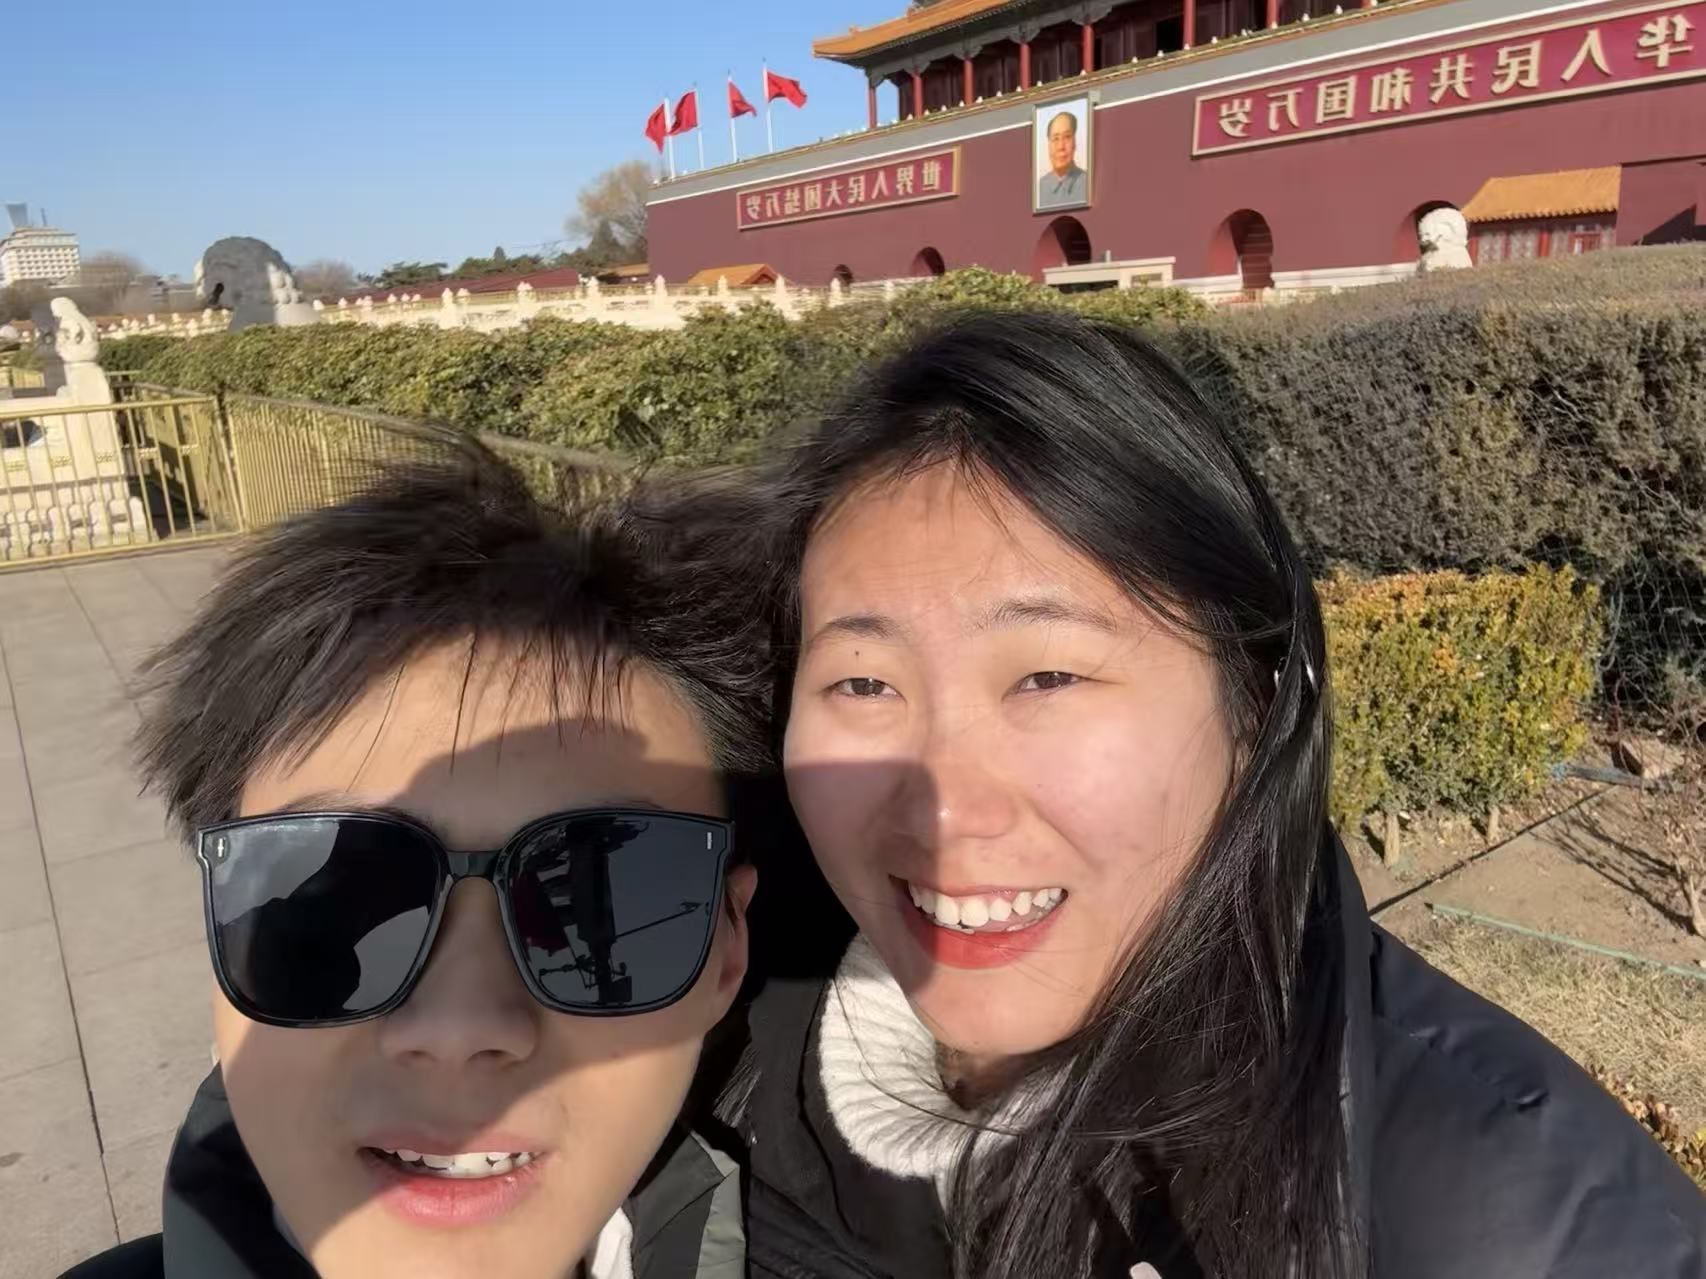
\includegraphics[width=\textwidth]{figures/articles/01-7.jpg}
        \caption*{\small{2024年2月29日于天安门广场}}
    \end{figure}
    那阵吹过我们一个下午的、自由的风，仿佛还跟在身后，诉说着一些关于永恒，却也关于此刻的私语。
\end{spacing}

\card{covers/cover6.jpg}{F}{永远支持你}{Forever support you}

\setstyle{Forever support you}

\subtitle{景山公园——红墙琉璃瓦叙事诗}

\large
\begin{spacing}{2}
    从天安门广场的恢弘与风中离开，我们像是从一段雄壮的乐章，步入了另一段舒缓的间奏。
    步入景山公园，那股庄严的、令人屏息的气息悄然散去，取而代之的是一种从容的静谧。

    那日的天气，当得起“春和景明”四字。阳光是温和的，不像午后那般炽烈，均匀地洒下来，
    像一层薄薄的、甜润的蜂蜜，涂抹在苍翠的古松与初萌的新芽上。空气里浮动着植物清新的气息，
    脚步踩在松软的土地上，声音都被吸了进去。

    \begin{figure}[!htbp]
        \centering
        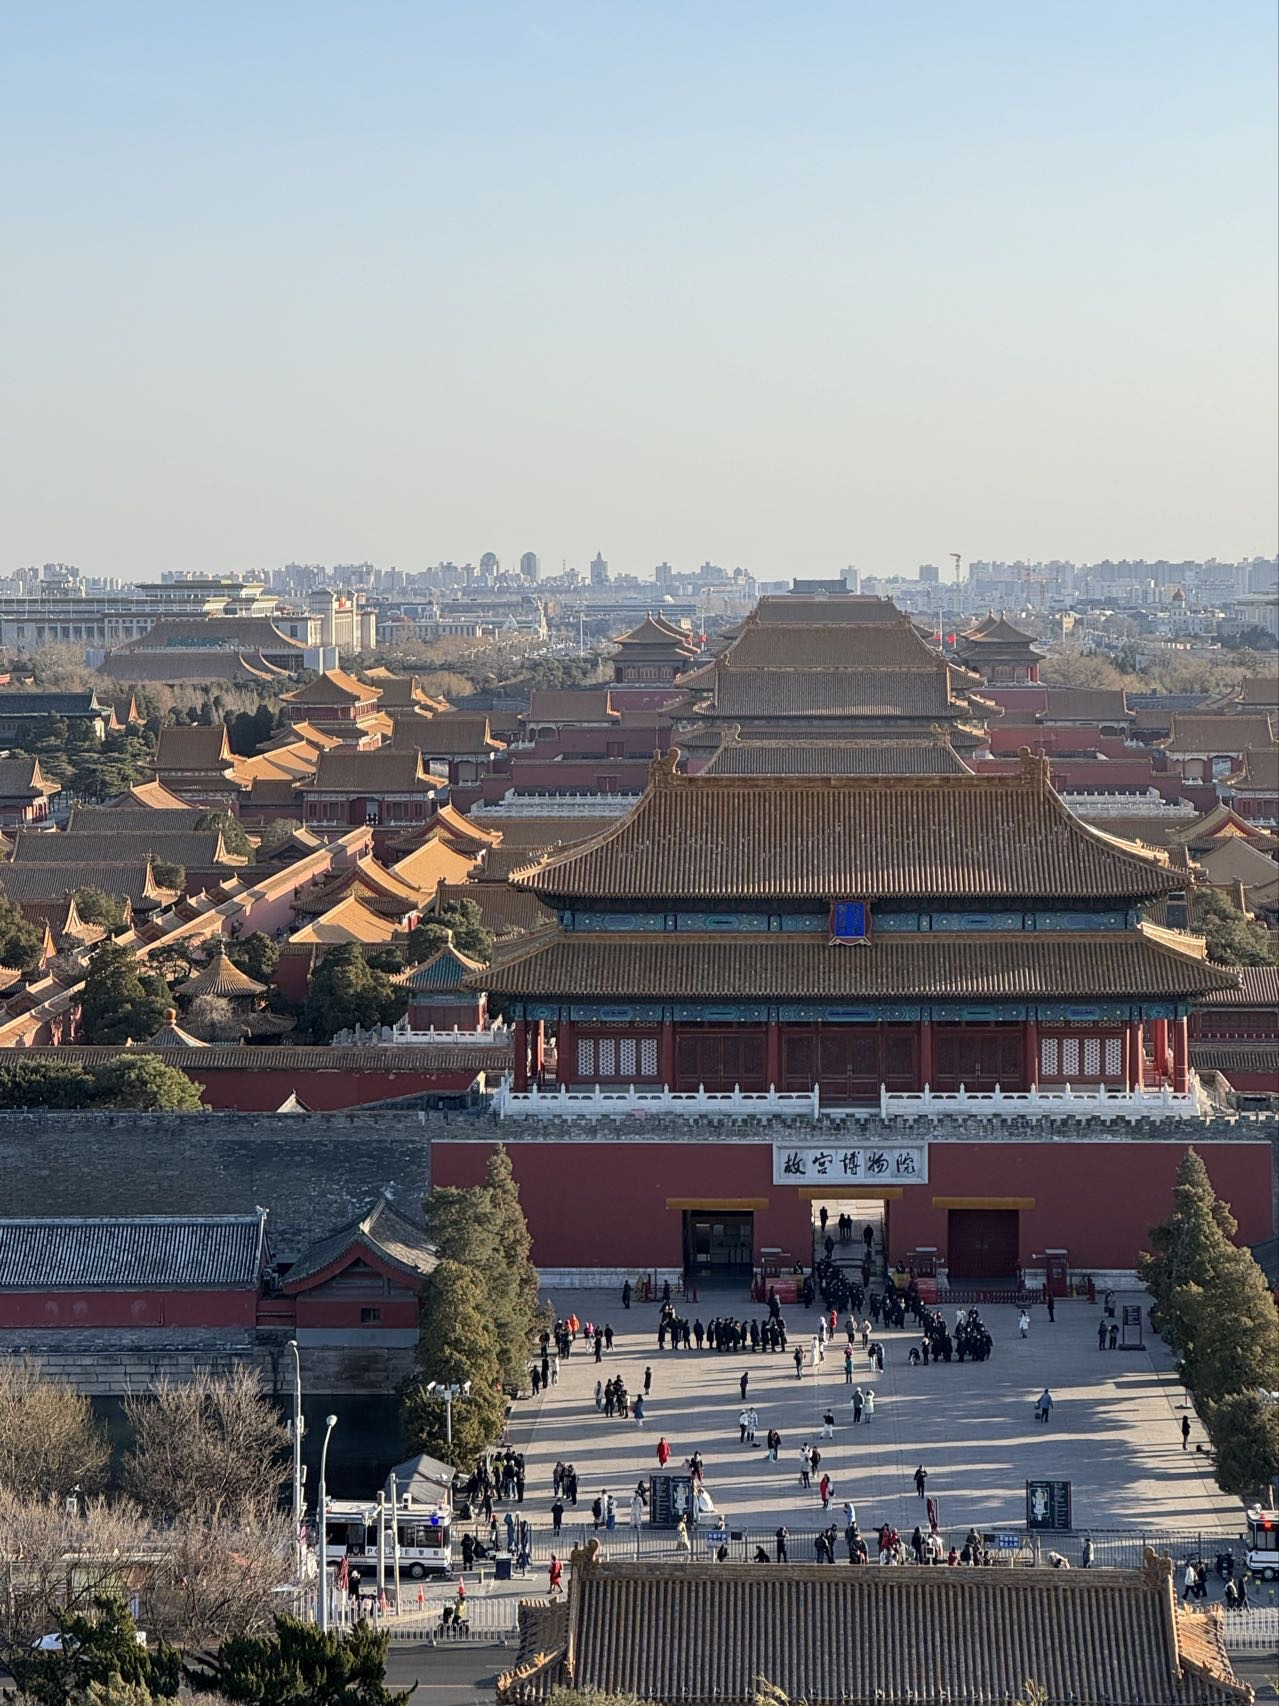
\includegraphics[width=0.5\textwidth]{figures/articles/01-8.jpg}
        \caption*{2024年2月29日于景山公园}
    \end{figure}

    我们沿着平缓的石阶向上，不疾不徐。穿过一重又一重的红墙，墙内是另一个世界。这里的红墙，
    不似故宫那般拒人千里的凛然，它更温厚，更亲近，墙头探出的枝桠，温柔地打破了规则的边界。
    登上万春亭的那一刻，风悄然静止，世界在眼前豁然铺展。没有预想中浓墨重彩的日落，
    天色是一种纯净的、渐变的蓝，从头顶的清透缓缓沉向天际的柔和。而脚下，
    便是那一片举世无双的盛景——整个紫禁城，毫无保留地袒露在我们眼前。

    你靠在我身边，手指轻轻指向太和殿那遥远的屋脊，阳光在你的侧脸勾勒出一圈柔和的光晕。
    我们没有说话，只是静静地看，看那鳞次栉比的殿顶，看那纵横交错的街巷，
    看时光在这座古老的城池里缓缓流淌。这一刻，不属于任何一个轰轰烈烈的朝代，
    它只属于这个春风和煦的傍晚，属于并肩俯瞰这座城市的我们。

    天色在不知不觉中，由清蓝转为静谧的灰蓝。脚下的“琥珀之城”亮起了星星点点的灯，像散落的星辰，
    与天际初生的晚星悄然呼应。我们转身下山，将那部无声的叙事诗留在了身后。但我知道，那首诗的某一页，已经用最温柔的笔触，
    记下了这个平静的春日，和一起读过它的我们。

    \begin{figure}[!htbp]
        \centering
        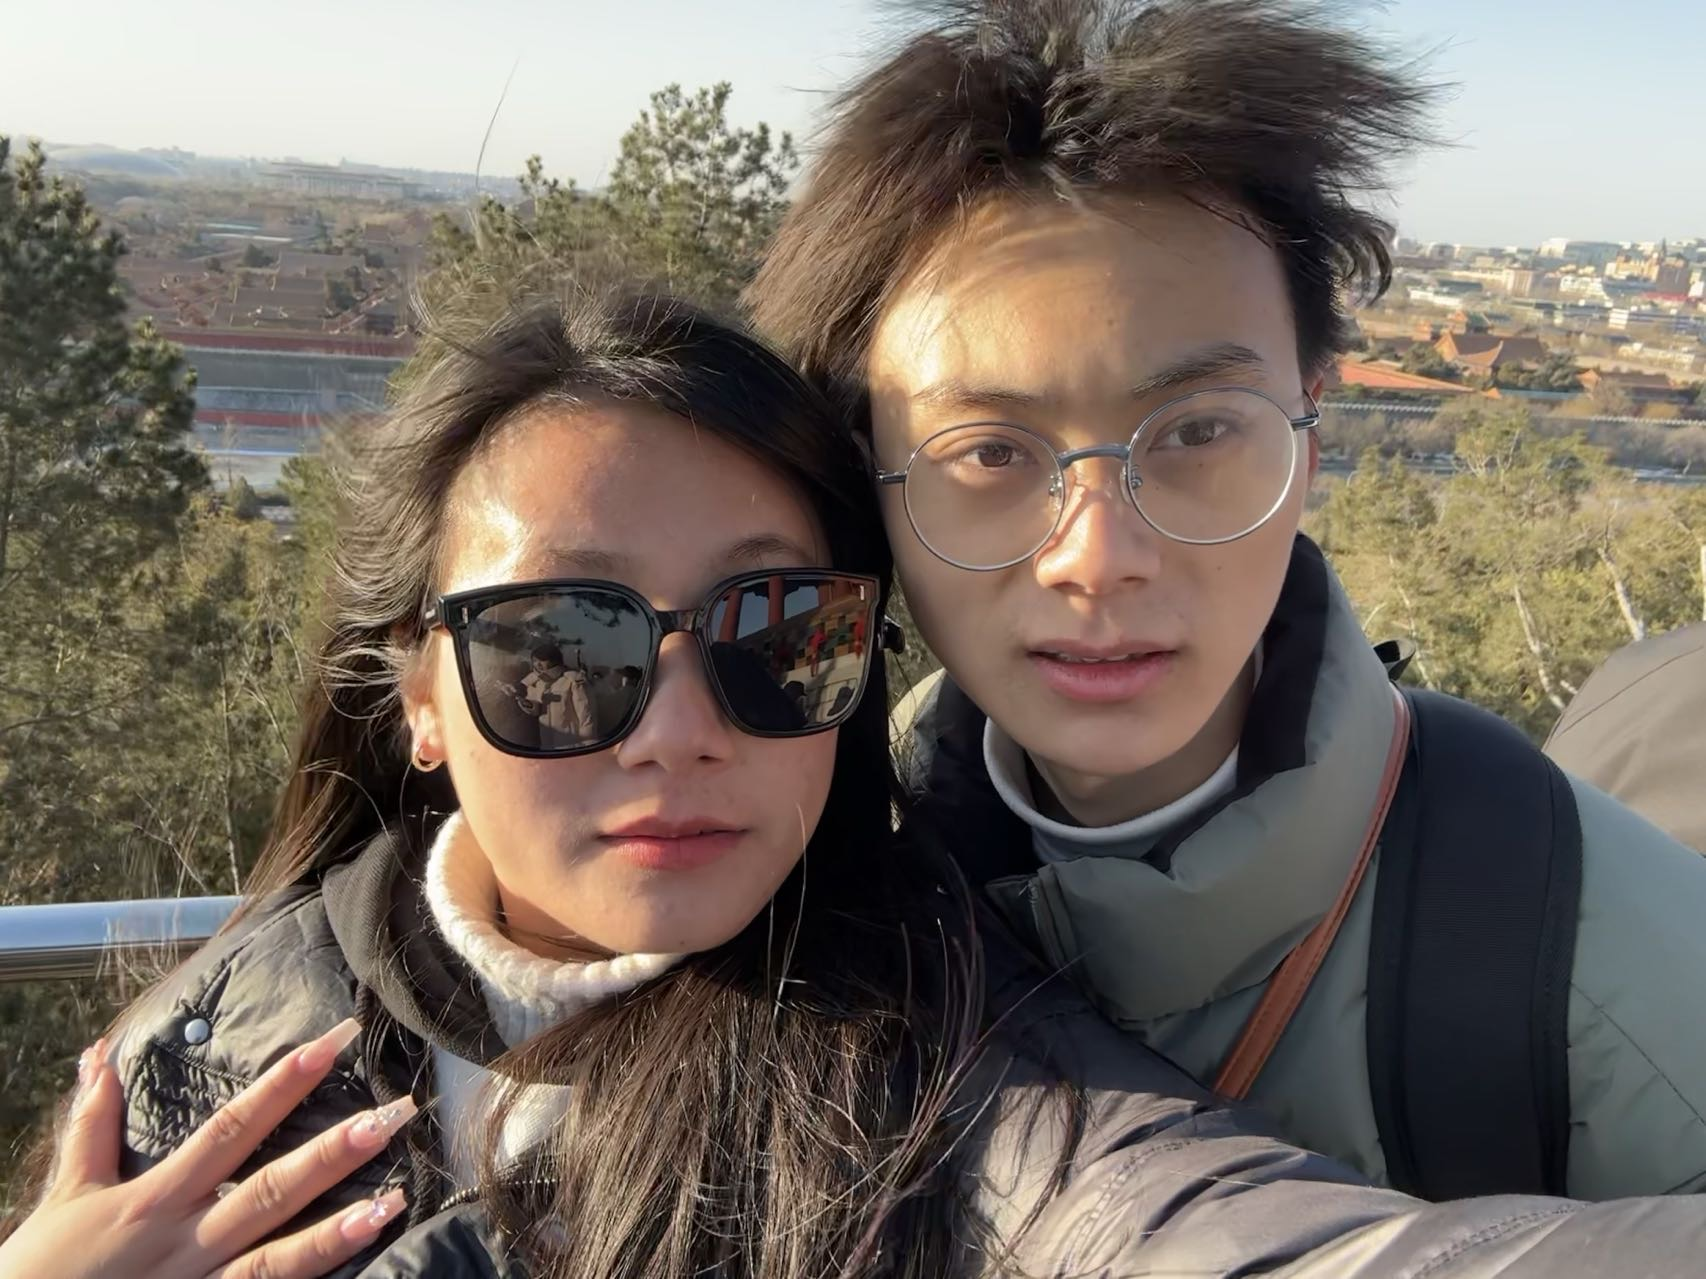
\includegraphics[width=\textwidth]{figures/articles/01-9.jpg}
        \caption*{2024年2月29日于景山公园}
    \end{figure}

    \bottomtext{“浮生若梦，为欢几何，唯你而已”}
\end{spacing}

\card{covers/cover7.jpg}{G}{给你一切你需要的}{Give you what you need}

\setstyle{Give you what you need}

\subtitle{天坛公园——天心石的回响}

\large
\begin{spacing}{2}
    那日的天坛，是被太阳烘焙透了的。三月的北京，春寒还未完全退去，但那一日的阳光却慷慨得如同盛夏，
    把每一块青石板都晒得发烫，空气里浮动着柏树和古木被炙烤后散发的醇厚香气。

    我们沿着漫长的神道向上走，影子在脚边缩成小小的一团。然后，我们走向那座被栏杆围起的、著名的圜丘。
    圜丘在无遮无拦的天空下，三层汉白玉台基在烈日下白得晃眼，像一座巨大的、通往苍穹的祭坛。
    阳光在石栏上跳跃，折射出刺目的光芒，让人几乎睁不开眼。我们一步步走上去，脚下石板的温热透过鞋底传来，
    那温度仿佛不是来自太阳，而是从历史的深处渗透而出。

    中心，便是那块天心石。它静静地躺在那里，光滑的表面反射着天光，像一只凝视苍穹的眼睛。传说站在上面轻声说话，
    声音会洪亮浑厚，能得到上天的回应。这个古老的传说让这块普通的石板变得神秘而庄严。四下里人热闹着，
    游客的谈笑声、相机的快门声、导游的讲解声交织在一起。你看着我，眼神里有一种鼓励。
    我深吸了一口灼热的空气，趁着人群暂时散去的空隙，走上前，独自站定在那块圆形的石板上。那一刻，
    时间仿佛静止了。头顶是浩瀚的蓝天，脚下是承载着无数祈愿的圣石，身边是注视着我的你。

    我没有呼喊，没有许下宏大的愿望，只是极轻地、用只有自己能听见的声音，念了你的名字。
    那声音轻得像一片羽毛落地，但在我的心里，它却重如千钧。在那一瞬间，我忽然明白了——上天不需要听见我的声音，
    因为我的整个世界，早已经被你的名字填满。

    \begin{figure}[!htbp]
        \centering
        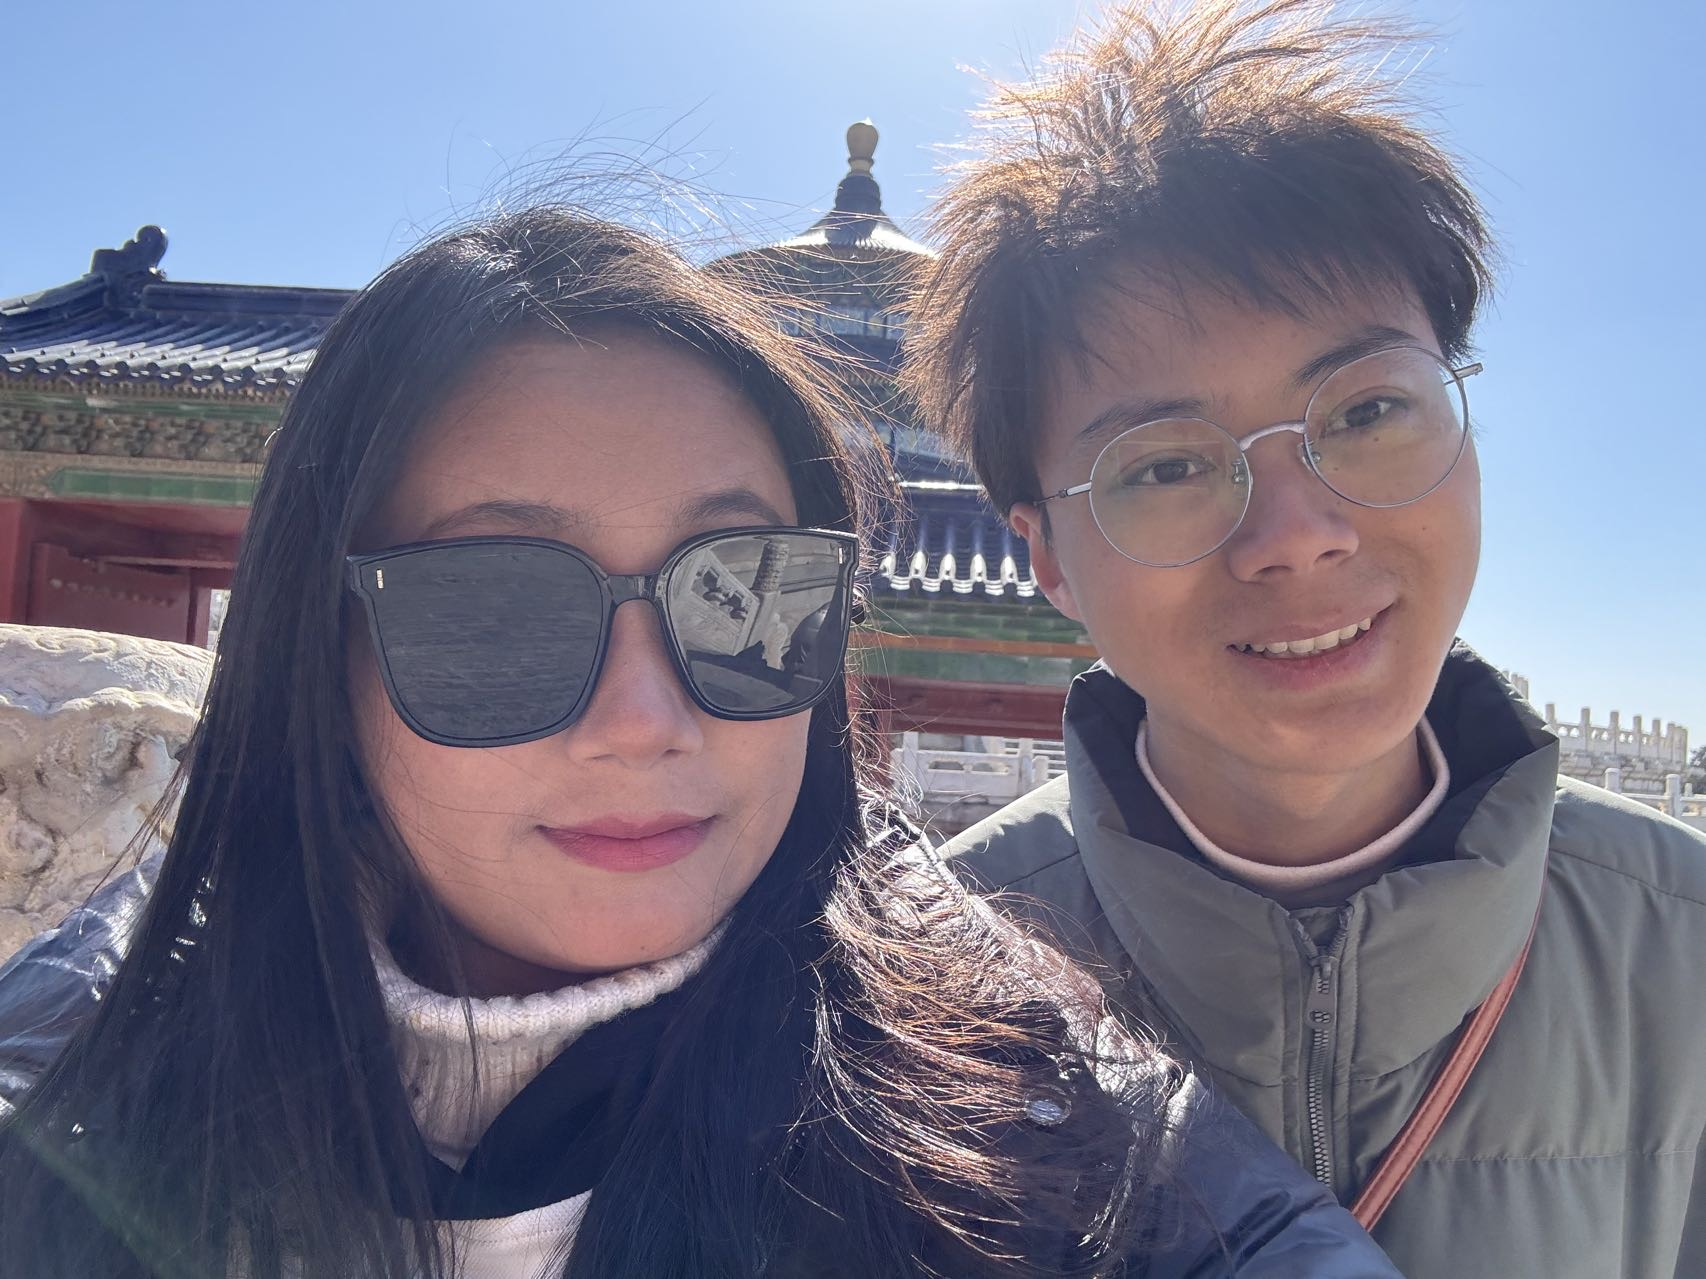
\includegraphics[width=0.8\textwidth]{figures/articles/01-10.jpg}
        \caption*{2024年3月1日于天坛公园}
    \end{figure}

    \bottomtext{“岁月为笔，相思入墨，字字皆是你”}
\end{spacing}
\clearpage